%---------------------------------------------------------------------------------
\chapter{Improvements to Aeronautical Waveforms}
\label{chap:improvements_waveforms}
%---------------------------------------------------------------------------------
\section{Introduction}
Techniques enabling efficiency gains in the utilization of the aeronautical spectrum were seen in Chapter \ref{chap:lit_review}. In particular, signal space diversity (SSD), i.e., modulation diversity, was discussed as a potential method to improve the reliability of A/G links. In this chapter, SSD is explored to address the spectrum efficiency of aeronautical communication systems. Specifically, an overview of the Quad State-Paired QPSK (QS-PQPSK) modulated signal \cite{tan2016quad}, noise and the different aeronautical channel models is presented. Thereafter, an evaluation of QS-PQPSK against D8PSK (used in the VDL-2 standard) under different aeronautical channel conditions is conducted. A Space-Time Block Coded QS-PQPSK (STBC QSPQPSK) in combination with STBC and QS-PQPSK is then proposed to further improve BER performance. An evaluation of the proposed STBC QS-PQPSK is also conducted against QS-PQPSK and D8PSK under various aeronautical channels to determine BER performance for various flight scenarios.

%%%%%%%%%%%%%%%%%%%%%%%%%%%%%%%%%%%%%%%%%%%%%%%%%%%%%%%%%%%%%%%%%%%%%%%%%%%%%%%%%%%%%%%%%%%%%%%%%%%%%%%%%%%%%%%%%%%%%%%%%%%%%%%%%%%%%%%%%
\section{Signal, Noise and Aeronautical Channel Model}

%%%%%%%%%%%%%%%%%%%%%%%%%%%%%%%%%%%%%%%%%%%%%%%%%%%%%%%%%%%%%%%%%%%%%%%%%%%%%%%%%%%%%%%%%%%%%%%%%%%%%%%%%%%%%%%%%%%%%%%%%%%%%%%%%%%%%%%%%
\subsection{Signal and Noise Model}

The signal representation of QS-PQPSK is briefly described in this section. In an earlier work \cite{tan2016quad} on the QSPQPSK modulation technique, data bits are grouped into blocks of 6 bits as $b_{i},...,b_{i+5} (i=0,6,12,...)$ transmitted over two symbol periods ($2T_{s}$), with additional data conveyed using one of two QPSK constellations as indices. The signal representation is seen in (\ref{QSPQPSK_eqn1}) to (\ref{QSPQPSK_eqn3}).

%%%%%%%%%%%%%%%%%%%%%%%%%%%%%%%%%%%%%%%%%%%%%%%%%%%%%%%%%%%%%%%%%%%%%%%%%%%%%%%%%
\begin{eqnarray} \label{QSPQPSK_eqn1}
S(t) =
  \begin{cases}
    S_1(t) &\quad 0<t\leq{T_s} \\
    S_2(t) &\quad T_s<t\leq{2T_s}\\
  \end{cases}
\end{eqnarray}
%%%%%%%%%%%%%%%%%%%%%%%%%%%%%%%%%%%%%%%%%%%%%%%%%%%%%%%%%%%%%%%%%%%%%%%%%%%%%%%%%
\begin{eqnarray} \label{QSPQPSK_eqn2}
S_1(t) = \sqrt{\frac{2E_s}{T_s}}\cos(2\pi{f_c}t-\phi(b_4))
\end{eqnarray}
%%%%%%%%%%%%%%%%%%%%%%%%%%%%%%%%%%%%%%%%%%%%%%%%%%%%%%%%%%%%%%%%%%%%%%%%%%%%%%%%%
\begin{eqnarray} \label{QSPQPSK_eqn3}
S_2(t) = \sqrt{\frac{2E_s}{T_s}}\cos(2\pi{f_c}t-\phi(b_5))
\end{eqnarray}
%%%%%%%%%%%%%%%%%%%%%%%%%%%%%%%%%%%%%%%%%%%%%%%%%%%%%%%%%%%%%%%%%%%%%%%%%%%%%%%%%
\begin{eqnarray} \label{QSPQPSK_eqn4}
\phi(b) = 
  \begin{cases}
    \frac{2\pi{m}}{4} & \quad \text{for } b = 0, \text{then } S_1 \text{or } S_2 \in Q_0 \\
    \frac{\pi(2m+1)}{4} & \quad \text{for } b = 1, \text{then } S_1 \text{or } S_2 \in Q_1 \\
  \end{cases}
\end{eqnarray}
%%%%%%%%%%%%%%%%%%%%%%%%%%%%%%%%%%%%%%%%%%%%%%%%%%%%%%%%%%%%%%%%%%%%%%%%%%%%%%%%%
where $m\in{0,1,2,3}$. The signals $S_1(t)$ and $S_2(t)$ each represent bits $b_i$, $b_{i+2}$ and bits $b_{i+2}$, $b_{i+3}$ respectively. The selected QPSK constellations and resultant phases of $S_1(t)$ and $S_2(t)$ are then selected by bits $b_{i+4}$ and $b_{i+5}$ correspondingly using (\ref{QSPQPSK_eqn4}). In this fashion, an effective 3 bits instead of two bits per symbol is transmitted per symbol period. The received signal in a fading channel can be represented as

%%%%%%%%%%%%%%%%%%%%%%%%%%%%%%%%%%%%%%%%%%%%%%%%%%%%%%%%%%%%%%%%%%%%%%%%%%%%%%%%%
\begin{eqnarray} \label{QSPQPSK_eqn5}
r(t) & = & S(t)\ast{h(t)} + n(t)
\end{eqnarray}
%%%%%%%%%%%%%%%%%%%%%%%%%%%%%%%%%%%%%%%%%%%%%%%%%%%%%%%%%%%%%%%%%%%%%%%%%%%%%%%%%
where $\ast$ denote convolution in time domain, $h(t)$ is the impulse response of the aeronautical communications channel and $n(t)$ represents Additive White Gaussian Noise (AWGN).

%%%%%%%%%%%%%%%%%%%%%%%%%%%%%%%%%%%%%%%%%%%%%%%%%%%%%%%%%%%%%%%%%%%%%%%%%%%%%%%%%%%%%%%%%%%%%%%%%%%%%%%%%%%%%%%%%%%%%%%%%%%%%%%%%%%%%%%%%

\subsection{Aeronautical Channel Models}
The A/G communication channels experienced by an aircraft can be categorized into en route, arrival/take-off, taxi and parking scenarios. These scenarios are summarized below, based on the paper by Haas \cite{haas2002aeronautical}.

%%%%%%%%%%%%%%%%%%%%%%%%%%%%%%%%%%%%%%%%%%%%%%%%%%%%%%%%%%%%%%%%%%%%%%%%%%%%%%%%%%%%%%%%%%%%%%%%%%%%%%%%%%%%%%%%%%%%%%%%%%%%%%%%%%%%%%%%%

\subsubsection{En route Scenario}
The en route scenario is present when an aircraft is maintaining A/G communications at cruising altitude with velocity taken as 440m/s. The en route scenario can be modelled as Rician fading for the Line-of-Sight (LOS) path with K factor $\approx$ 15dB and Rayleigh fading for non Line-of-Sight (NLOS) i.e. multipath components.

%%%%%%%%%%%%%%%%%%%%%%%%%%%%%%%%%%%%%%%%%%%%%%%%%%%%%%%%%%%%%%%%%%%%%%%%%%%%%%%%%%%%%%%%%%%%%%%%%%%%%%%%%%%%%%%%%%%%%%%%%%%%%%%%%%%%%%%%%

\subsubsection{Arrival/Take-off Scenario}

The arrival/take-off scenario is present when an aircraft is maintaining A/G communications during the landing or takeoff phase of a flight, with velocity taken as 150m/s. Both the LOS and NLOS components can also be modelled as Rician and Rayleigh fading respectively with K factor $\approx$ 15dB for the LOS component.

%%%%%%%%%%%%%%%%%%%%%%%%%%%%%%%%%%%%%%%%%%%%%%%%%%%%%%%%%%%%%%%%%%%%%%%%%%%%%%%%%%%%%%%%%%%%%%%%%%%%%%%%%%%%%%%%%%%%%%%%%%%%%%%%%%%%%%%%%

\subsubsection{Taxi Scenario}
The taxi scenario occurs when an aircraft is maintaining airport/tarmac communications whilst transiting from runway to terminal and vice versa. The velocity of the aircraft is taken as 15m/s with LOS and NLOS components modelled as Rician and Rayleigh fading respectively. In this scenario, the airport is assumed to be situated in a rural area with K factor $\approx$ 6.9dB for the LOS component.

%%%%%%%%%%%%%%%%%%%%%%%%%%%%%%%%%%%%%%%%%%%%%%%%%%%%%%%%%%%%%%%%%%%%%%%%%%%%%%%%%%%%%%%%%%%%%%%%%%%%%%%%%%%%%%%%%%%%%%%%%%%%%%%%%%%%%%%%%

\subsubsection{Parking Scenario}
The parking scenario ensues when an aircraft is parked or moving (maximum velocity of 5.5m/s) near a terminal whilst maintaining airport/tarmac communications. In this scenario, LOS communications can be assumed absent due to LOS obstructions from surrounding airport buildings thus only multipath Rayleigh fading is considered.

%%%%%%%%%%%%%%%%%%%%%%%%%%%%%%%%%%%%%%%%%%%%%%%%%%%%%%%%%%%%%%%%%%%%%%%%%%%%%%%%%%%%%%%%%%%%%%%%%%%%%%%%%%%%%%%%%%%%%%%%%%%%%%%%%%%%%%%%%
\section{Performance of QS-PQPSK in Aeronautical Communication Channels}

The simulated BER performance of QS-PQPSK and D8PSK (VDL-2) are compared under the various aeronautical channels mentioned earlier. In particular, the average BER performance of 1000 trials were taken, with full channel state information (CSI) assumed for the various scenarios. 

The BER performance of QS-PQPSK and D8PSK in the en route and arrival/take-off scenarios are seen in Fig. \ref{fig:chap3_fig1} and Fig. \ref{fig:chap3_fig2} respectively. One LOS path and one Non-LOS path i.e. Rician fading with one Rayleigh fading component as multipath was considered for the en route scenario. Similarly, one LOS and three NLOS paths were considered for the arrival/take-off scenario. In both scenarios, QS-PQPSK outperformed D8PSK, especially at high SNRs.

\begin{figure} []
\centering
%\vspace{-1.5in}
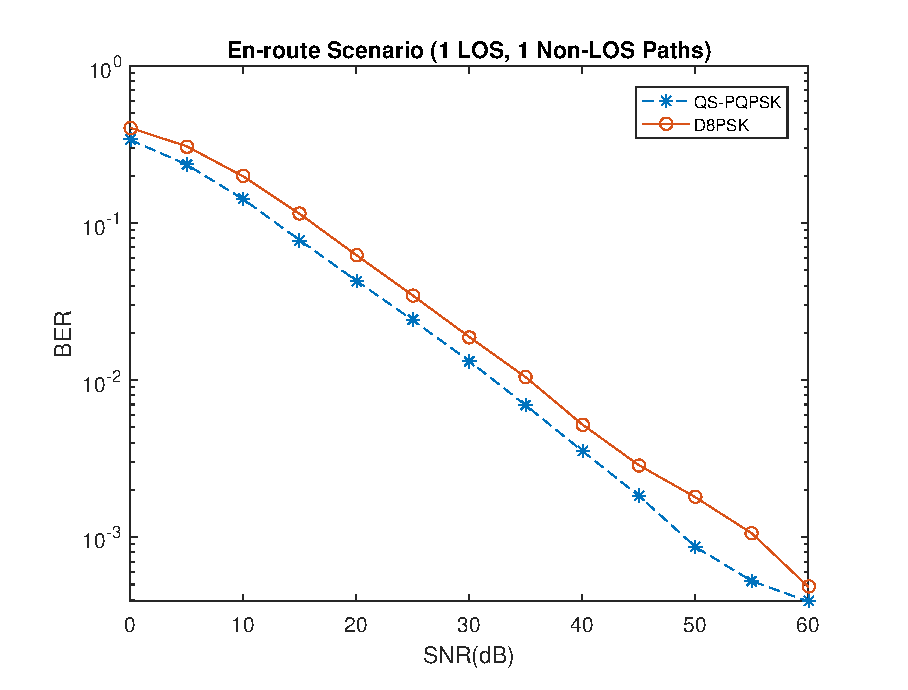
\includegraphics [width=0.5\columnwidth]{chap3_fig/chap3_fig1.eps} 
%\vspace{-1.5in}
\caption{BER performance of QS-PQPSK and D8PSK (En route).}
\label{fig:chap3_fig1}
\end{figure}

\begin{figure} []
\centering
%\vspace{-1.5in}
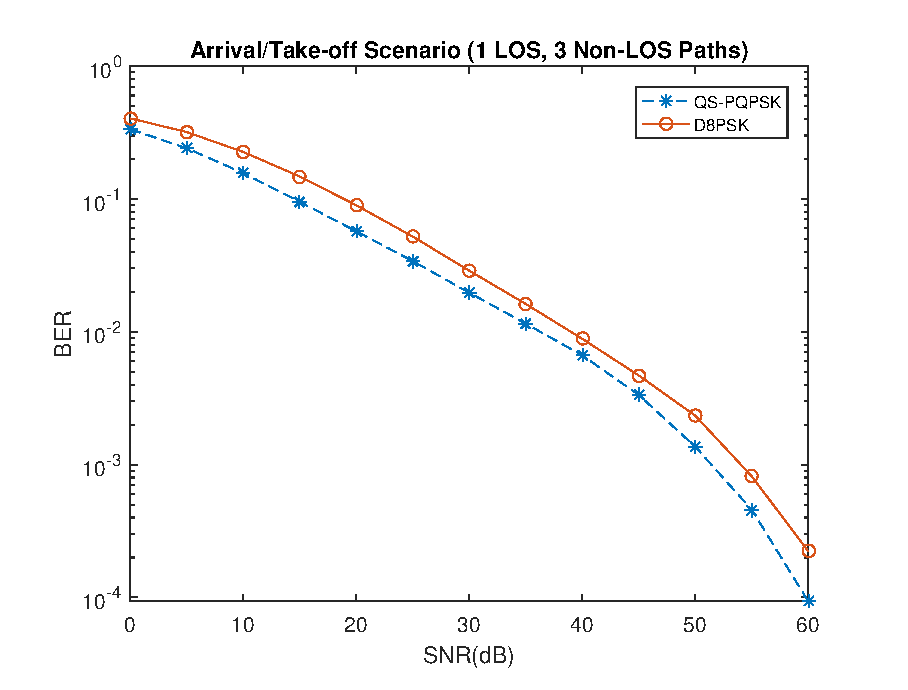
\includegraphics [width=0.5\columnwidth]{chap3_fig/chap3_fig2.eps} 
%\vspace{-1.5in}
\caption{BER performance of QS-PQPSK and D8PSK (Arrival/Take-off).}
\label{fig:chap3_fig2}
\end{figure}

The BER performance of QS-PQPSK and D8PSK in the taxi scenario is seen in Fig. \ref{fig:chap3_fig3}. In this scenario, LOS communication is simulated between the moving aircraft on the ground and the airport ground station, with five reflected paths modeled as Rayleigh fading components. It can be observed that the QS-PQPSK outperforms D8PSK, especially at higher SNRs of 30dB. Likewise, the BER performance of QS-PQPSK and D8PSK in the parking scenario is seen in Fig. \ref{fig:chap3_fig4}. In the parking scenario, non-LOS communication is simulated between the stationary aircraft and the airport ground station i.e. the aeronautical channel is modeled as a Rayleigh fading channel with seven NLOS paths. This is because a parked aircraft could be blocked from LOS view from the ground station. Similar to the trends seen in Fig. \ref{fig:chap3_fig1} to Fig. \ref{fig:chap3_fig3}, the performance of QS-PQPSK is observed to be superior to D8PSK for various SNRs. From Fig. \ref{fig:chap3_fig1} to Fig. \ref{fig:chap3_fig4}, it can also be seen that QS-PQPSK outperforms D8PSK under all scenarios and could improve efficiency.

\begin{figure} []
\centering
%\vspace{-1.5in}
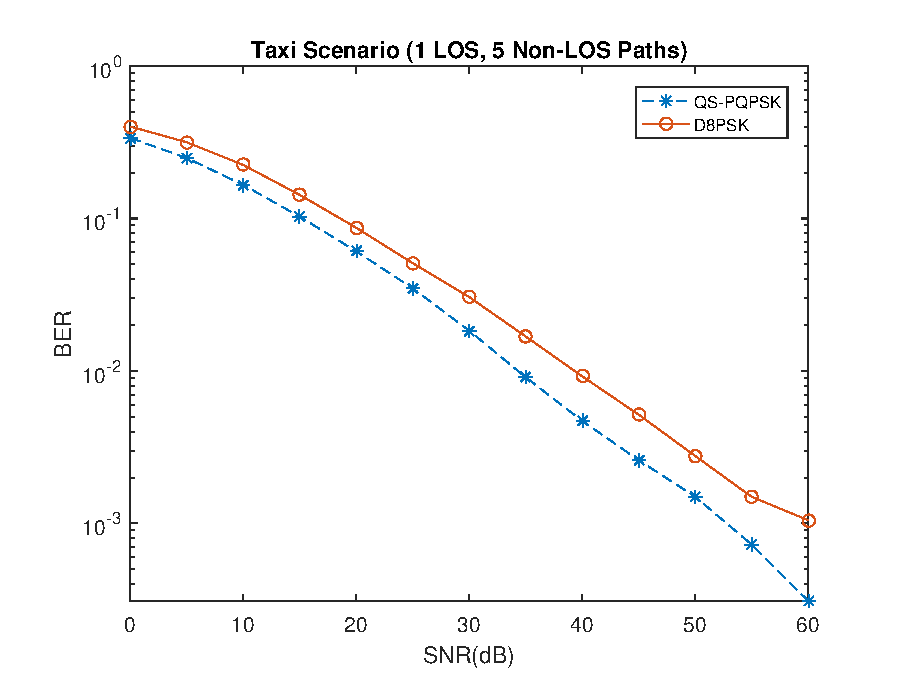
\includegraphics [width=0.5\columnwidth]{chap3_fig/chap3_fig3.eps} 
%\vspace{-1.5in}
\caption{BER performance of QS-PQPSK and D8PSK (Taxi).}
\label{fig:chap3_fig3}
\end{figure}

\begin{figure} []
\centering
%\vspace{-1.5in}
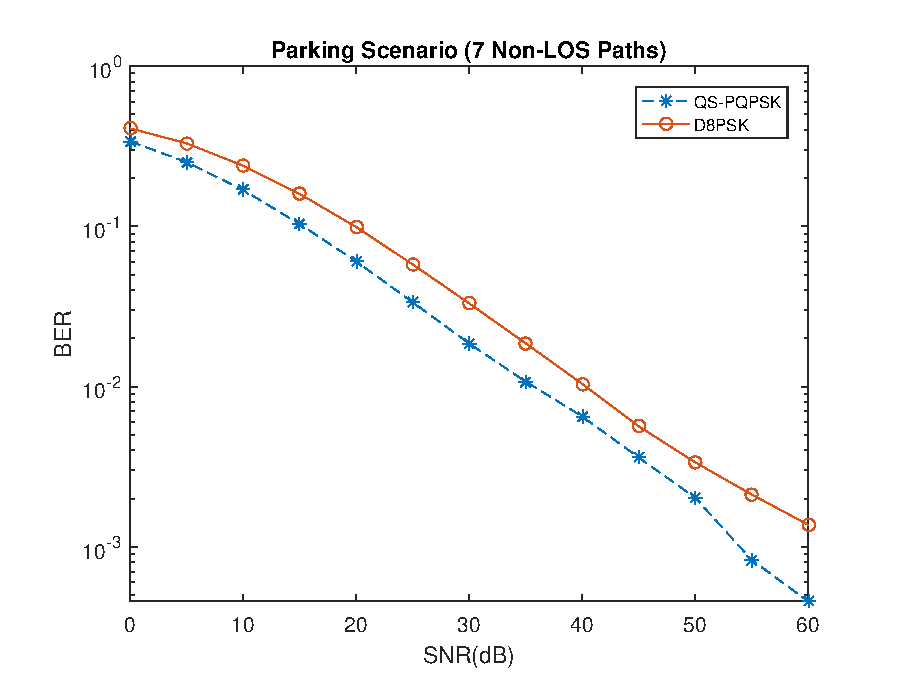
\includegraphics [width=0.5\columnwidth]{chap3_fig/chap3_fig4.eps} 
%\vspace{-1.5in}
\caption{BER performance of QS-PQPSK and D8PSK (Parking).}
\label{fig:chap3_fig4}
\end{figure}



%%%%%%%%%%%%%%%%%%%%%%%%%%%%%%%%%%%%%%%%%%%%%%%%%%%%%%%%%%%%%%%%%%%%%%%%%%%%%%%%%%%%%%%%%%%%%%%%%%%%%%%%%%%%%%%%%%%%%%%%%%%%%%%%%%%%%%%%%
\section{Performance of STBC QS-PQPSK in Aeronautical Communication Channels}

The Space Time Block Code (STBC) scheme described by Alamouti \cite{alamouti1998simple} has had a positive impact in wireless communications, with multiple works done in this direction. In essence, Alamouti proposed a two-transmit, one-receive antenna and a two-transmit, two-receive antenna scheme for transmit diversity. In this section, STBC QSPQPSK (Fig. \ref{fig:chap3_fig5}) is proposed by combining the former (two-transmit, one-receive antenna scheme) with QS-PQPSK to further improve BER performance. The proposed method is only simulated and evaluated for air-to-ground (A/G) communication. But the scheme can be extended to ground-to-air (G/A) communication also, the concept of which is outlined below.

%%%%%%%%%%%%%%%%%%%%%%%%%%%%%%%%%%%%%%%%%%%%%%%%%%%%%%%%%%%%%%%%%%%%%%%%%%%%%%%%%%%%%%%%%%%%%%%%%%%%%%%%%%%%%%%%%%%%%%%%%%%%%%%%%%%%%%%%%
\subsection{A/G Communications}
Let $S_i$, $h_i$, $n_i$ and $\ast$ denote the $i^{th}$ QS-PQPSK symbol, $i^{th}$ antenna path gain, $i^{th}$ complex AWGN and the complex conjugate operation respectively. After modulating the outgoing binary data into symbols $S_i$, the symbols are transmitted via two transmit antennas, on the aircraft, simultaneously over two symbol periods ($2T_S$) to the ground station receive antenna. To aid in explaining the concept of the proposed scheme, consider the transmission of the first two symbols $S_1$ and $S_2$ seen in Table \ref{table:chap3_table1} \cite{alamouti1998simple}.

\begin{figure} [!htpb]
\centering
\vspace{-1.5in}
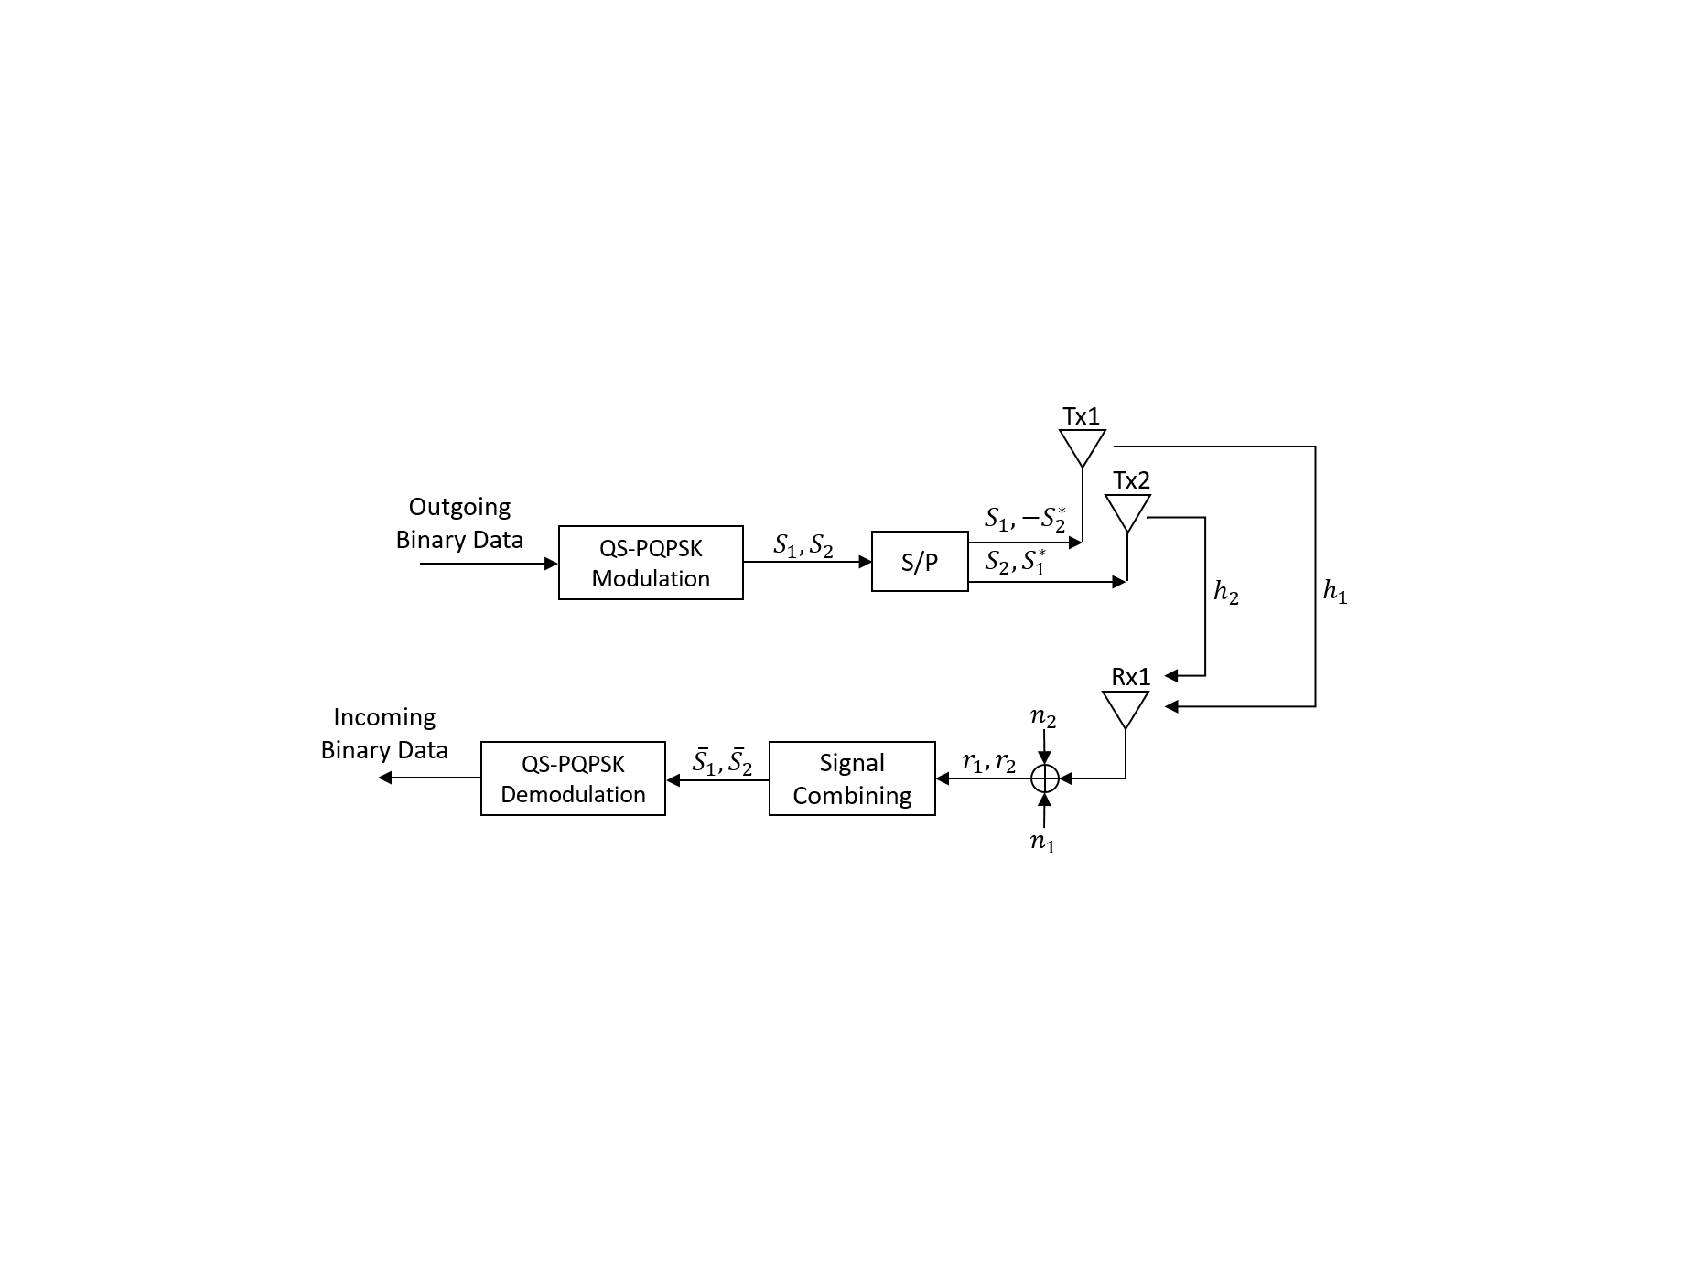
\includegraphics [width=1\columnwidth]{chap3_fig/chap3_fig5.eps} 
\vspace{-1.5in}
\caption{Proposed STBC QS-PQPSK two-transmit, one-receive antenna scheme.}
\label{fig:chap3_fig5}
\end{figure}

\begin{table}[]
\centering
\caption{Symbol Transmission of the Proposed STBC QS-PQPSK Scheme}
\label{table:chap3_table1}
\begin{tabular}{ccc}
\hline
\textbf{Time $t$} & \textbf{Antenna Tx1} & \textbf{Antenna Tx2} \\ \hline \hline
 $0 < t \leq T_s$& $S_1$ & $S_2$            \\ 
 $0 < t \leq T_s$& $-S_2^{\ast}$ & $S_1^{\ast}$            \\ \hline
\end{tabular}
\end{table}

The received signal over $2T_S$ for $0$ $<$ $t$ ${\leq}$ $T_s$ can be written as
%%%%%%%%%%%%%%%%%%%%%%%%%%%%%%%%%%%%%%%%%%%%%%%%%%%%%%%%%%%%%%%%%%%%%%%%%%%%%%%%%
\begin{eqnarray} \label{QSPQPSK_eqn6}
r(t) = r_1 = S_1{h_1} + S_2{h_2} + n_1
\end{eqnarray}
\begin{eqnarray} \label{QSPQPSK_eqn7}
r(t + T_s) = r_2 = S_1^{\ast}{h_2} - S_2^{\ast}{h_1} + n_2.
\end{eqnarray}
%%%%%%%%%%%%%%%%%%%%%%%%%%%%%%%%%%%%%%%%%%%%%%%%%%%%%%%%%%%%%%%%%%%%%%%%%%%%%%%%%

Let $\overline{S_1}$ and $\overline{S_2}$ represent the recovered symbols $S_1$ and $S_2$ respectively. To recover both symbols, $r_1$ and $r_2$ are combined using $h_1$ and $h_2$ (assuming full CSI) as
%%%%%%%%%%%%%%%%%%%%%%%%%%%%%%%%%%%%%%%%%%%%%%%%%%%%%%%%%%%%%%%%%%%%%%%%%%%%%%%%%
\begin{eqnarray} \label{QSPQPSK_eqn8}
\overline{S_1} = r_1{h_1^{\ast}} + r_2^{\ast}{h_2}
\end{eqnarray}
\begin{eqnarray} \label{QSPQPSK_eqn9}
\overline{S_2} = r_1{h_2^{\ast}} - r_2^{\ast}{h_1}
\end{eqnarray}
%%%%%%%%%%%%%%%%%%%%%%%%%%%%%%%%%%%%%%%%%%%%%%%%%%%%%%%%%%%%%%%%%%%%%%%%%%%%%%%%%

Substituting (\ref{QSPQPSK_eqn6}) and (\ref{QSPQPSK_eqn7}) into (\ref{QSPQPSK_eqn8}) and (\ref{QSPQPSK_eqn9}) leads to
%%%%%%%%%%%%%%%%%%%%%%%%%%%%%%%%%%%%%%%%%%%%%%%%%%%%%%%%%%%%%%%%%%%%%%%%%%%%%%%%%
\begin{eqnarray} \label{QSPQPSK_eqn8}
\overline{S_1} = \left(\left|h_1\right|^2 + \left|h_2\right|^2\right)S_1 + n_1h_1^{\ast} + n_2^{\ast}h_2
\end{eqnarray}
\begin{eqnarray} \label{QSPQPSK_eqn9}
\overline{S_2} = \left(\left|h_1\right|^2 + \left|h_2\right|^2\right)S_2 + n_1h_2^{\ast} - n_2^{\ast}h_1
\end{eqnarray}
%%%%%%%%%%%%%%%%%%%%%%%%%%%%%%%%%%%%%%%%%%%%%%%%%%%%%%%%%%%%%%%%%%%%%%%%%%%%%%%%%

After $S_1$ and $S_2$ have been recovered, the QS-PQPSK symbols are demodulated to recover the incoming binary data as seen in Fig. \ref{fig:chap3_fig5}.

\begin{figure} []
\centering
%\vspace{-1.5in}
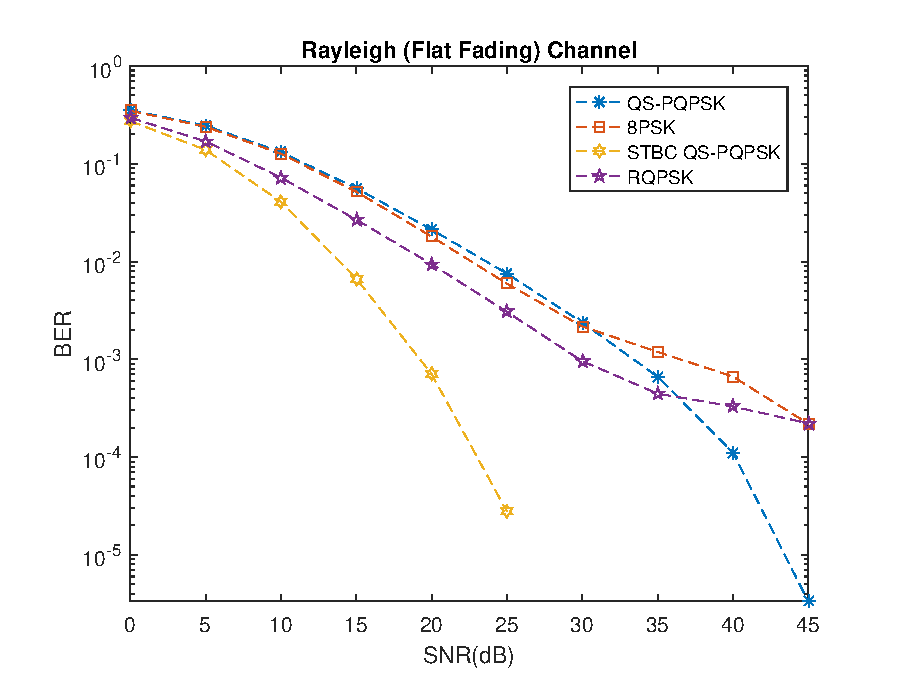
\includegraphics [width=0.5\columnwidth]{chap3_fig/chap3_fig6.eps} 
%\vspace{-1.5in}
\caption{BER performance of STBC QS-PQPSK, QS-PQPSK, 8PSK and
RQPSK in Rayleigh flat fading channel.}
\label{fig:chap3_fig6}
\end{figure}

In Fig. \ref{fig:chap3_fig6}, a similar comparison, as in \cite{tan2016quad}, of the BER performance (average of 1000 trials with known CSI) of the proposed STBC QS-PQPSK against QS-PQPSK, 8PSK and RQPSK \cite{liu1992rotative} in Rayleigh flat fading channel is shown. It can be observed that the BER performance of QS-PQPSK was further improved when combined with STBC i.e. STBC QS-PQPSK and is evident, even at low SNRs of 5dB.

%%%%%%%%%%%%%%%%%%%%%%%%%%%%%%%%%%%%%%%%%%%%%%%%%%%%%%%%%%%%%%%%%%%%%%%%%%%%%%%%%%%%%%%%%%%%%%%%%%%%%%%%%%%%%%%%%%%%%%%%%%%%%%%%%%%%%%%%%
\subsection{G/A Communications}
It should be noted that the proposed scheme was evaluated for A/G communication. However, the scheme can also be extended for the ground to aircraft communication. This could be realized using a similar two-transmit, one-receive antenna system (Fig. \ref{fig:chap3_fig5}), by incorporating either Time Division Duplex (TDD) or Frequency Division Duplex (FDD) into the proposed STBC QS-PQPSK scheme (Fig. \ref{fig:chap3_fig7}). In fact, TDD has been adopted for use in VDL2 \cite{stacey2008aeronautical} and LDACS2 \cite{neji2013survey} while FDD has been seen in LDACS1 \cite{neji2013survey}. These methods can similarly be applied for the proposed STBC QS-PQPSK scheme for both Air-to-Ground and Ground-to-Air links. Specifically, TDD STBC QS-PQPSK will entail the use of two antennas on both the aircraft and ground station (Fig. \ref{fig:chap3_fig7}a). Under such an arrangement, both aircraft and ground stations are allocated dedicated timeslots for A/G and G/A communications. Alternatively, separate frequency channels for A/G and G/A links can be dedicated via FDD STBC QSPQPSK (Fig. \ref{fig:chap3_fig7}b). Both the TDD and FDD arrangements seen in Fig. \ref{fig:chap3_fig7} do have its own merits and limitations. In the former (Fig. \ref{fig:chap3_fig7}a), the scheduling of timeslots for both A/G and G/A communications will result in half-duplex communication. However, less bandwidth is required and additional antennas will not be needed. In case of FDD STBC QS-PQPSK, the
communication is full duplex, but additional antennas and frequency channels will be required.

\begin{figure} []
\centering
\vspace{-1.0in}
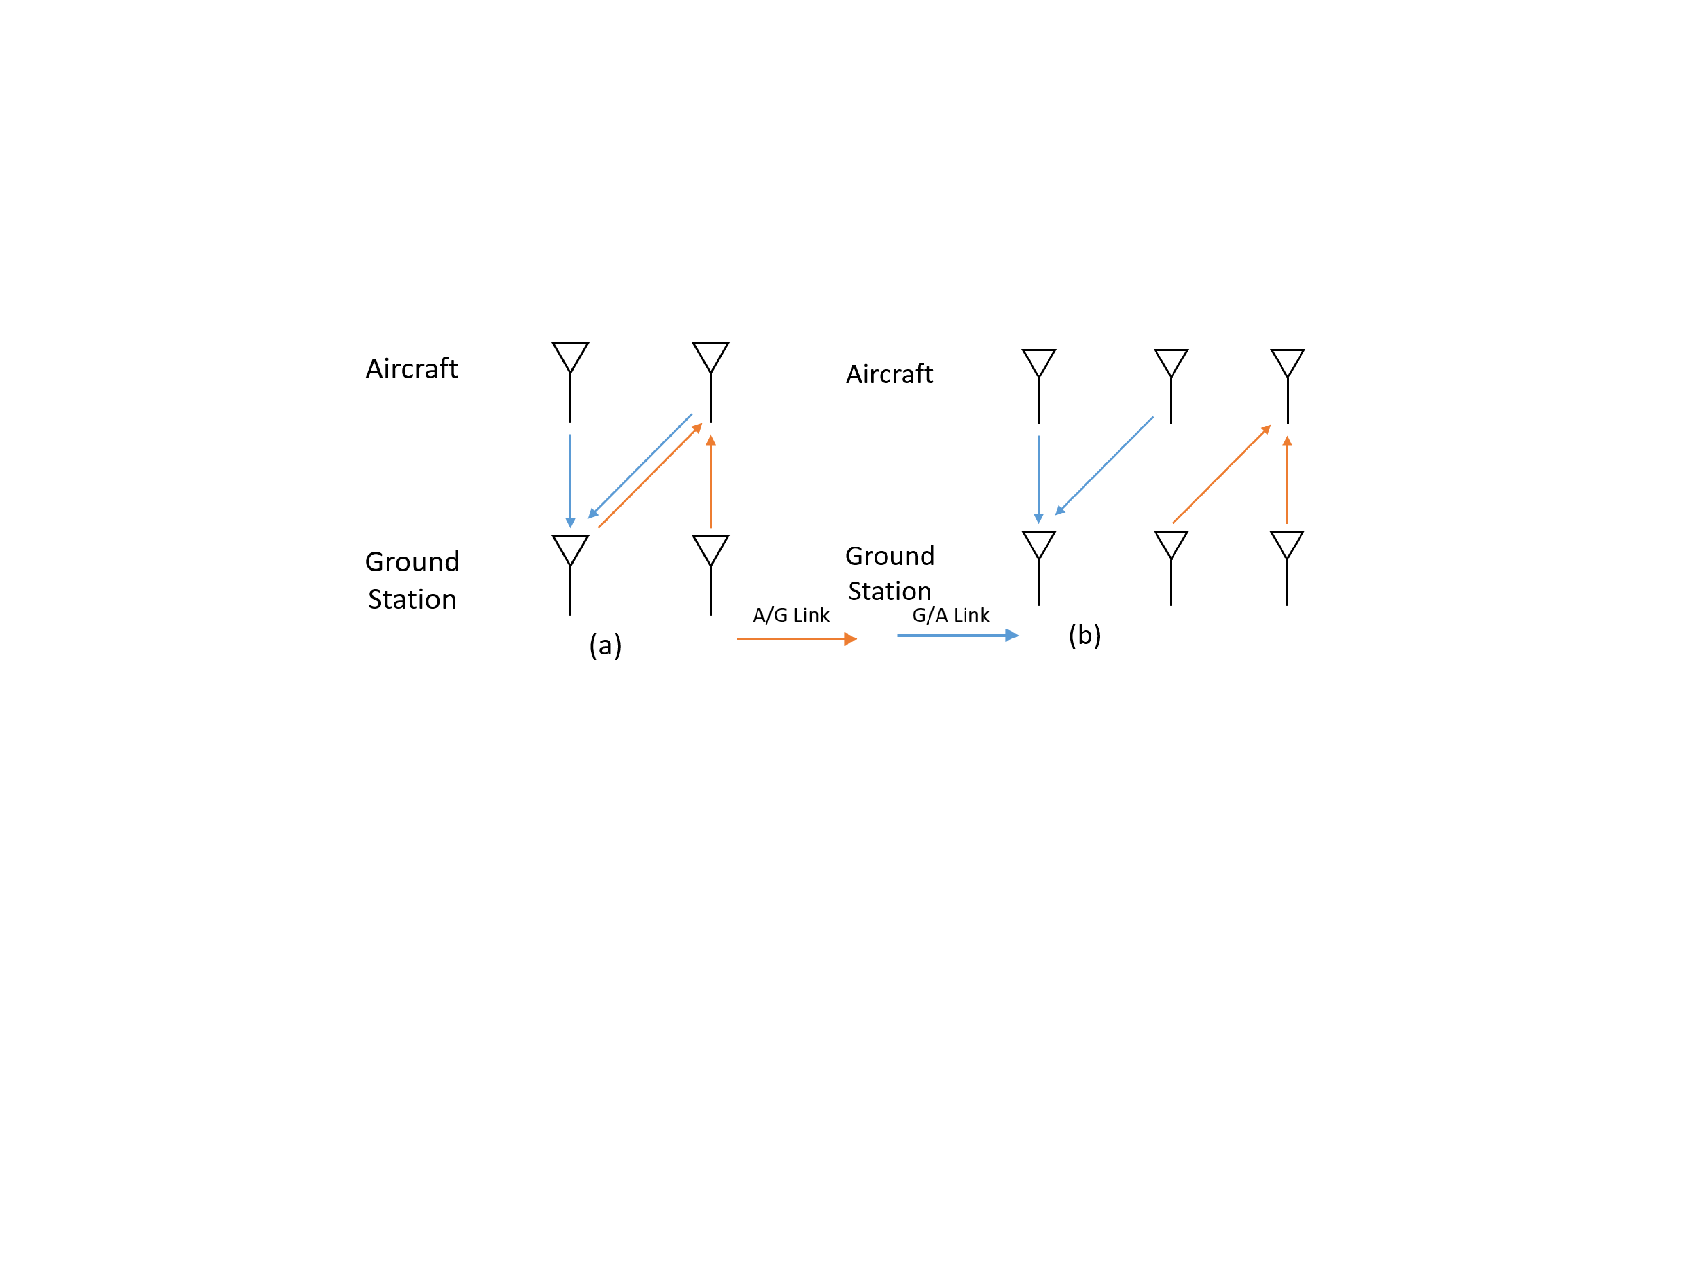
\includegraphics [width=1\columnwidth]{chap3_fig/chap3_fig7.eps} 
\vspace{-2.5in}
\caption{TDD (a) and FDD (b) based communications for the proposed
STBC QS-PQPSK scheme.}
\label{fig:chap3_fig7}
\end{figure}


In this section, simulation results for the STBC QSPQPSK are given for the special case of one path (LOS or NLOS) for the different aeronautical channel models. These are preliminary results in the formulation of STBC QSPQPSK, and further work is ongoing to handle more multipath scenarios. The performance of STBC QS-PQPSK is compared against QS-PQPSK and D8PSK under the same aeronautical channel conditions. The average BER of 1000 trials were taken for each channel condition simulated, with full CSI assumed.

\begin{figure}[]
\centering
%\vspace{-1.0in}
\includegraphics[width=1\columnwidth]{chap3_fig/chap3_fig8.eps}
\vspace{-2.in}
\caption{BER performance of STBC QS-PQPSK, QS-PQPSK and D8PSK in both en route (left) and arrival/take-off (right) scenarios.}
\label{fig:chap3_fig8}
\end{figure}

The proposed STBC QS-PQPSK scheme is compared against QS-PQPSK and D8PSK in both en route and arrival/take-off scenarios (Fig. \ref{fig:chap3_fig8}). In both scenarios, LOS A/G communications is simulated between the flying aircraft and a ground station, with the aeronautical channel modeled as a Rician fading channel. It can be observed that STBC QS-PQPSK outperforms both QS-PQPSK and D8PSK in both en route and arrival/take-off scenarios, even at low SNRs. The BER performance of STBC QS-PQPSK, QS-PQPSK and D8PSK in the taxi scenario is seen in Fig. \ref{fig:chap3_fig9}. In this scenario, LOS communications is simulated between the moving aircraft on the ground and the airport ground station, with STBC QS-PQPSK having superior BER performance at low SNR despite a lower K factor of 6.9dB in this scenario.

\begin{figure} []
\centering
%\vspace{-1.5in}
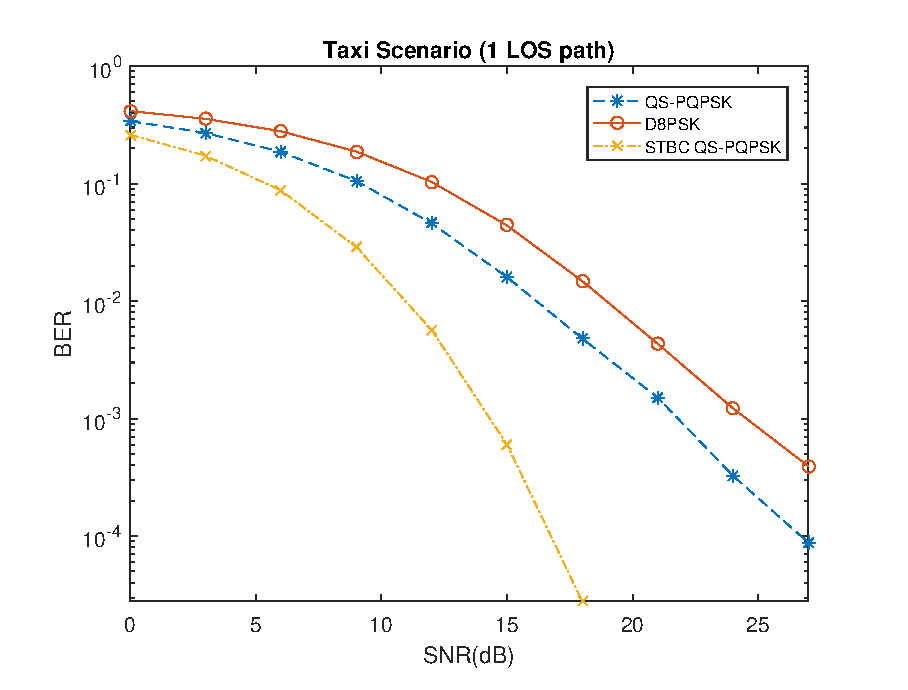
\includegraphics [width=0.5\columnwidth]{chap3_fig/chap3_fig9.eps} 
%\vspace{-1.5in}
\caption{BER performance of STBC QS-PQPSK, QS-PQPSK and D8PSK in the taxi scenario.}
\label{fig:chap3_fig9}
\end{figure}

\begin{figure} []
\centering
%\vspace{-1.5in}
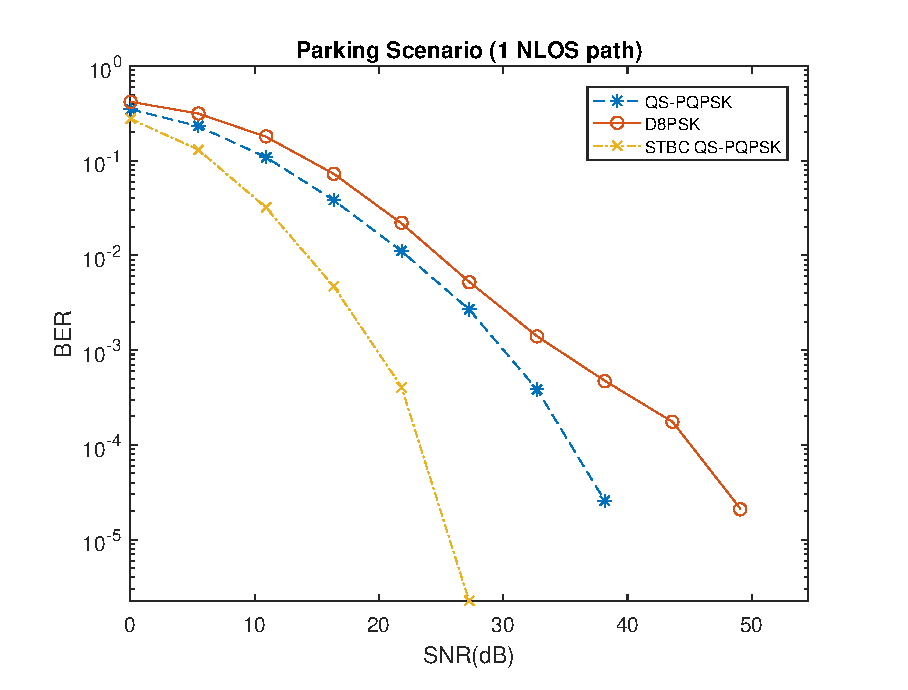
\includegraphics [width=0.5\columnwidth]{chap3_fig/chap3_fig10.eps} 
%\vspace{-1.5in}
\caption{BER performance of STBC QS-PQPSK, QS-PQPSK and D8PSK in the parking scenario.}
\label{fig:chap3_fig10}
\end{figure}

The BER performance of STBC QS-PQPSK, QS-PQPSK and D8PSK in the parking scenario is seen in Fig. \ref{fig:chap3_fig10}. Non-LOS communications is simulated between the stationary aircraft and airport ground station in this scenario, with the aeronautical channel modeled as a Rayleigh flat fading channel. It is observed that in the parking scenario, STBC QSPQPSK exhibits better BER performance even at low SNRs. It can also be observed that the BER performance of STBC QSPQPSK is consistently superior than QS-PQPSK and D8PSK under the various simulated aeronautical channel models, highlighting the suitability of STBC QS-PQPSK for A/G communications.

%%%%%%%%%%%%%%%%%%%%%%%%%%%%%%%%%%%%%%%%%%%%%%%%%%%%%%%%%%%%%%%%%%%%%%%%%%%%%%%%%%%%%%%%%%%%%%%%%%%%%%%%%%%%%%%%%%%%%%%%%%%%%%%%%%%%%%%%%
\section{Summary}
As a consequence of air travel growth, the move towards an efficient avionic architecture and suitable efficient waveform is a necessity. In this regard, this chapter addresses the spectral efficiency of the communication waveform. The Quad State-Paired QPSK (QS-PQPSK), a more spectrally efficient modulation scheme proposed in our previous work, was compared against D8PSK (VDL-2) under various aeronautical communication channels. Simulations showed that QSPQPSK BER performance outclassed D8PSK under all simulated scenarios. To further improve the efficiency of aeronautical waveforms, a new modulation scheme called the Space Time Block Coded QS-PQPSK (STBC QS-PQPSK) was proposed for A/G communications. Simulations also showed STBC QS-PQPSK having superior BER performance under all simulated scenarios when compared against QSPQPSK and D8PSK, underscoring STBC QS-PQPSK as a suitable efficient aeronautical waveform.







